\chapter{}

Havia ainda outro motivo para eu não querer deixar Araraquara naquele momento, ainda que eu continuasse a detestar a cidade.
E esse motivo era  meu pai.
Em 1974, ele foi submetido a uma das primeiras cirurgias de colocação de pontes de safena no coração feitas no país.
Era uma técnica pioneira na época, muito invasiva e, nas palavras do meu pai, para o paciente equivalia a ser “atropelado por um caminhão”.
O fato é que, após essa operação que o salvou de um enfarte iminente do miocárdio, ele nunca mais voltou a ter uma vida normal.
Era perseguido por uma dor anginosa constante, “uma espada de Dâmocles erguida sobre a cabeça”, como ele a descrevia, a lembrá-lo de que a solução fora apenas paliativa.
A doença continuava a progredir na sua agourenta caminhada.
Até porque ele se recusava a seguir as recomendações médicas para deixar de fumar e beber e recomeçou a fazê-lo às escondidas ainda durante o período de recuperação.
 Na tentativa de afastá-lo de uma rotina que parecia deprimi-lo cada vez mais, minha mãe tinha aceitado até a ideia de apoiá-lo na compra de um sítio próximo da cidade, (ela que jurara jamais voltar a pôr os pés num) onde, de alguma maneira, ele podia retornar às suas raízes de homem do campo.

Durante algum tempo, a compra do sítio pareceu cumprir a função esperada.
Tornou-se um lugar para reunir a família e os amigos nos fins de semana.
Ele ficava feliz vendo as crianças brincando na terra, comendo fruta no pé, convivendo com os primos.
De novo, comprou uma Kombi e, no sábado, levantava animado com a perspectiva de abarrotá-la com as compras de comida e bebida para o churrasco semanal.
Para ajudar nas despesas de manutenção, o sítio ganhou um pomar de laranjas que era o orgulho dele.
 Durante a semana, fugia um dia ou outro para ver a plantação que o divertia bem mais que o ruído das máquinas da fábrica.

Havia ainda outro motivo para eu não querer deixar Araraquara naquele momento, ainda que eu continuasse a detestar a cidade.
E esse motivo era  meu pai.
Em 1974, ele foi submetido a uma das primeiras cirurgias de colocação de pontes de safena no coração feitas no país.
Era uma técnica pioneira na época, muito invasiva e, nas palavras do meu pai, para o paciente equivalia a ser “atropelado por um caminhão”.
O fato é que, após essa operação que o salvou de um enfarte iminente do miocárdio, ele nunca mais voltou a ter uma vida normal.
Era perseguido por uma dor anginosa constante, “uma espada de Dâmocles erguida sobre a cabeça”, como ele a descrevia, a lembrá-lo de que a solução fora apenas paliativa.
A doença continuava a progredir na sua agourenta caminhada.
Até porque ele se recusava a seguir as recomendações médicas para deixar de fumar e beber e recomeçou a fazê-lo às escondidas ainda durante o período de recuperação.
 Na tentativa de afastá-lo de uma rotina que parecia deprimi-lo cada vez mais, minha mãe tinha aceitado até a ideia de apoiá-lo na compra de um sítio próximo da cidade, (ela que jurara jamais voltar a por os pés num) onde, de alguma maneira, ele podia retornar às suas raízes de homem do campo.

Durante algum tempo, a compra do sítio pareceu cumprir a função esperada.
Tornou-se um lugar para reunir a família e os amigos nos fins de semana.
Ele ficava feliz vendo as crianças brincando na terra, comendo fruta no pé, convivendo com os primos.
De novo, comprou uma Kombi e, no sábado, levantava animado com a perspectiva de abarrotá-la com as compras de comida e bebida para o churrasco semanal.
Para ajudar nas despesas de manutenção, o sítio ganhou um pomar de laranjas que era o orgulho dele.
 Durante a semana, fugia um dia ou outro para ver a plantação que o divertia bem mais que o ruído das máquinas da fábrica.

\begin{figure}
\centering
\includegraphics[width=0.6\linewidth]{27/papai+mamãe.png}
\caption{Papai e mamãe na construção do sítio.}
\end{figure}

\begin{figure}
\centering
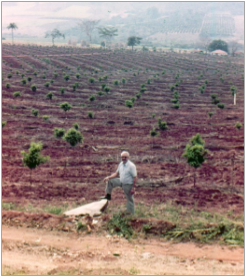
\includegraphics[width=0.6\linewidth]{27/papai+laranjal.png}
\caption{Papai e o laranjal em formação.}
\end{figure}

Meu cunhado Renato tornou-se a alma do lugar.
Engraçado, comilão e gozador, assumia a churrasqueira assessorado pelo maior amigo do papai, o Rubinho Lombardi, outro grande pândego.
Vivemos ali grandes histórias, festas, Natais, aniversários, batizados.
Papai não concebia outro destino para todo mundo nos fins de semana e se aborrecia quando alguém desertava.
Assim, o programa acabou por tornar-se meio compulsório, a ponto de Paulo defini-lo como “estado de sítio” e papai, que o decretava, acabou virando por extensão, o “Comandante”.
Ninguém foi mais beneficiada que eu pela existência daquele lugar.
Nos fins de semana em que Paulo não estava, que eram muitos, era lá que eu tinha um descanso, pois os cuidados com a criançada ficavam socializados entre todos.
Eram nove primos, com idades muito próximas e que conviveram tanto nesse período que custa acreditar que hoje sejam tão distantes.

\begin{figure}
\hfill
\centering
\begin{subfigure}[h]{0.4\linewidth}
    \centering
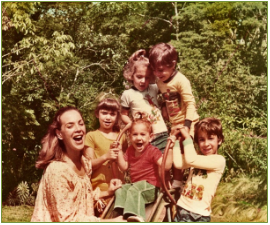
\includegraphics[width=\linewidth]{27/primos-1.png}
\end{subfigure}
\hfill
\begin{subfigure}[h]{0.4\linewidth}
    \centering
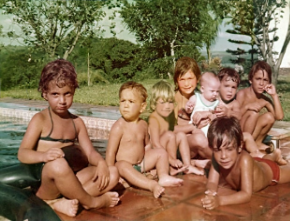
\includegraphics[width=1\linewidth]{27/primos-2.png}
\end{subfigure}
\caption{Os primos reunidos no sítio.}
\end{figure}

\begin{figure}
\centering
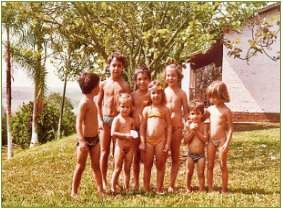
\includegraphics[width=0.6\linewidth]{27/primos-maiores.png}
\caption{Os primos, já maiores, nas férias.}
\end{figure}

\begin{figure}
\centering
\includegraphics[width=0.6\linewidth]{27/paulo+crianças.png}
\caption{Paulo e as crianças na carrocinha.}
\end{figure}

\begin{figure}
\centering
\includegraphics[width=0.6\linewidth]{27/renatão.png}
\caption{Renatão.}
\end{figure}

\begin{figure}
\centering
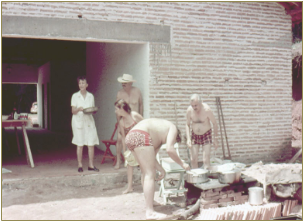
\includegraphics[width=0.6\linewidth]{27/improviso.png}
\caption{Vó Didi, Papai, Binho Lombardi e Renato improvisando um almoço no sítio.}
\end{figure}

O sítio mereceria, ele só, um livro para contar as histórias que dele ficaram.
Em torno da mesa da copa, por anos, varamos a noite conversando, trocando experiências, rindo, partilhando dramas.
Fomos uma família, na acepção da palavra.
Ele desbancou até mesmo o apartamento do Guarujá, outra aquisição do papai que nos permitia frequentar o mar, outra das paixões dele.


Porém, com a passagem do tempo e a progressão inexorável da doença, já não sabíamos se o sítio passara a fazer bem ou mal ao Comandante.
Ele se cansava muito facilmente, o esforço de percorrer o laranjal e subir o morro até a mina d’água, como ele gostava de fazer pela manhã, provocava-lhe a angina e, consciente do seu estado, meu pai, ao que parece, decidiu apressar o fim.
Ele, que nunca bebia durante o dia, no sítio começava logo cedo.
Segurava numa das mãos a lata de cerveja e, na outra, o indefectível cigarro.
E se enfurecia se alguém tentasse dissuadi-lo.


Hoje, olhando para trás, me pergunto onde minha mãe e eu buscamos resistência para enfrentar esse período. 
Tenho dificuldade até mesmo para lembrar em detalhes o que aconteceu.
Só me lembro que Nabhia, a professora de Matemática incumbida de elaborar o horário do Colégio em que eu lecionava, privilegiava-me com um horário especial que distribuía minhas obrigatórias vinte e cinco aulas semanais entre as manhãs e as tardes, alternadamente, de modo que eu pudesse estar presente o máximo tempo possível em casa, junto das quatro crianças.
Ao mesmo tempo, era cada vez mais necessário que eu desse apoio a mamãe na assistência ao meu pai.
Como é comum acontecer nestas situações, ele, à medida que piorava, voltava sua irritação contra ela, a ponto de que havia noites em que mamãe vinha dormir com as crianças, enquanto eu tomava o lugar dela, indo dar plantão no apartamento deles.
Por alguma razão, naquele dias difíceis, eu era uma das poucas pessoas que meu pai parecia atender.
Com meu irmão mais velho, o relacionamento nunca fora bom.
Maria Lúcia, minha irmã era, na época, impulsiva e imatura demais para segurar o tranco.
João partiria para uma viagem de intercâmbio aos Estados Unidos e, pouco depois de voltar, passaria no vestibular para Medicina, indo estudar em São Paulo.
Paulinho era um adolescente ainda e partiria ele também, em breve, para uma experiência de intercâmbio nos Estados Unidos, como o irmão.

Papai tinha cada vez mais dificuldade para dormir.
Os calmantes somados à bebida e ao cigarro pareciam, ao contrário, excitá-lo e ele varava madrugadas fumando sem parar.
Na janela da sala, de pijama, cigarro entre os dedos, ele parecia entregue a uma revisão de vida sem fim, vez ou outra passando a mão pelos cabelos, falando sozinho, preso de uma angústia sem remédio.
No sítio, era debruçado sobre a balaustrada da varanda que eu ia encontrá-lo, madrugada alta, fumando um cigarro atrás do outro.
Às vezes Martha, uma grande amiga deles, outra fumante inveterada, vinha lhe fazer companhia, às vezes o Rubinho ou a mulher dele, Yolanda, outras vezes eu.
Mas, vencidos pelo cansaço acabávamos indo dormir e ele ficava.
No dia seguinte, levantávamos acabados e ele, milagrosamente acordava em forma, pronto para recomeçar.
Durante a semana, na cidade, era para a fábrica que ele ia para abri-la pontualmente às sete horas, como fez por trinta e três anos sem falhar, até morrer.


De enorme ajuda nesse período foi meu cunhado, Renato.
Ele era outra pessoa que meu pai acatava e a quem ele queria como filho.
E que, como filho, apanhava também suas sobras quando meu pai se revoltava.
O Comandante, apesar das pontes de safena, teve pelo menos mais quatro enfartes antes daquele que o matou e ainda dois edemas pulmonares, e em todas as internações que se sucederam a esses eventos, Renato revezou com mamãe e comigo nas duras noites em claro.
Uma dívida impagável.


Os momentos de distensão, eu os passava com as crianças.
Levava-os diariamente a passear nas praças da cidade.
Era o meu refrigério, mas festa mesmo era quando o Paulo estava para chegar.
Como eles esperavam esse momento! Vindo uma vez a cada mês, Paulo não era o pai que chegava.
Era um amigo, era o irmão mais velho, era o que vinha para brincar com eles, levá-los passear, viajar, que nunca ficava bravo, que inventava mil e uma novidades para distrai-los.
Disso decorreu a confusão que ficou: nenhum deles o chama de pai, até hoje.
No início, todos me chamavam de mãe.
De repente, os mais velhos, percebendo alguma incoerência, passaram a me chamar de Teresa.
E os mais novos, Fernando, Paula e Vicente me chamam de mãe até agora e ao pai, de Paulo.
Se eu ficasse brava, mesmo não gostando, admitiam.
Bronca do pai, porém, era mágoa certa e inaceitável.